\vspace{1em}
\begin{center}PzIA\end{center}
\hrule
\vspace{1em}


\textbf{Ecco che l'azione si intensifica!} Un agente giace a terra in difficoltà colpito da Laura, mentre l'altro si lancia al loro inseguimento. Il suo drone sfreccia attraverso i corridoi del QM diretto all'inseguimento delle due fuggiasche che puntano alla \textit{Classical Control Unit}. \emph{Attenzione!} Un segnale di comunicazione improvviso fa gelare il sangue nelle vene dell'altro agente.

Dal centro di controllo, il Supervisore osserva la scena con freddezza implacabile. La sua voce, trasmessa senza traccia di empatia, rompe il silenzio nel canale privato degli agenti:

\begin{quote}
\enquote{Non tollero fallimenti.}
\end{quote}

\textbf{Colpo di scena!} Con un semplice comando, il Supervisore disattiva l'agente in difficoltà. La sua sagoma svanisce istantaneamente dal sistema, eliminata con l'efficienza impietosa del protocollo. \emph{Un'azione drastica che alza la posta in gioco!}

L'agente superstite, testimone della sorte del suo compagno, è colto da un'ondata di terrore. \emph{Sa che non può permettersi errori!} Determinato a evitare la stessa fine, accelera, inseguendo Laura e Marley con precisione letale. \textbf{La tensione è alle stelle!}

\section{Il Drone \textit{CH4}}

Laura guida il drone \textit{CH4} con una destrezza sorprendente!
Sta per lasciare il QM per dirigersi vero la CCU ma deve attraversare il dielettrico del condensatore.

Il suo sguardo è determinato. Non c'è incertezza. Deve attraversare il dielettrico. Ecco che Laura prepara il suo drone per evitare che interagisca con il campo elettrico accumulato. Attenzione, è un momento cruciale: il condensatorea è carico, come una molla pronta a scattare. Ogni movimento sbagliato potrebbe provocare un arco elettrico devastante!

Laura regola la velocità del drone, impostando con precisione il livello di isolamento dei rotori. \textit{Perfetto, sta calcolando il punto d'ingresso.} Ecco che il drone si avvicina al confine del dielettrico. Gli strumenti a bordo stanno analizzando le proprietà del campo elettrico—un lavoro di millisecondi, ma ogni dato conta.

E ora… ora accelera! Il drone CH4 si lancia nel dielettrico. L’aria sembra vibrare attorno al campo elettrico; una leggera scarica illumina il percorso del drone. Tutto si svolge in una frazione di secondo: Laura tiene saldamente i comandi, corregge la traiettoria al volo. Sta dosando con precisione chirurgica il flusso di energia attraverso i circuiti del drone per evitare sovraccarichi.

Ma attenzione! Un lieve squilibrio nel campo! Il drone trema, i sensori segnalano un picco di tensione! Laura risponde prontamente, modificando l’angolo di rotazione dei rotori. Una mossa audace, perfettamente sincronizzata. Il drone attraversa il dielettrico in un lampo di luce.


\begin{tcolorbox}[colback=gray!5,colframe=gray!80,title=\textbf{Scheda Informativa}]
\begin{itemize}
    \item \textbf{Luogo}: \emph{Classical Control Unit}
    \item \textbf{Giorno e ora}: Il tempo non è osservabile
    \item \textbf{Situazione}: Laura e Marley puntano verso la QCE.
\end{itemize}
\end{tcolorbox}


\textit{È incredibile! Ce l'ha fatta!} Laura emerge dall’altra parte del condensatore con una traiettoria impeccabile. Il drone è intatto, i sensori segnalano la stabilità ripristinata. Gli osservatori non osservano per non influenzare le traiettorie e Laura non si concede il lusso di rilassarsi.

Sta già pianificando il prossimo passo, un altro ostacolo da superare nel labirinto della Classical Control Unit. Un’impresa straordinaria, un controllo assoluto: Laura dimostra ancora una volta che nulla può fermarla.

Che momento epico!


Ogni componente rappresenta un ostacolo: chip integrati, condensatori, minuscole resistenze che formano una vera e propria giungla elettronica. Ma Laura li evita con precisione millimetrica, sfruttando la sua conoscenza approfondita dei circuiti. \textbf{È una vera maestra del volo!}

Con il cuore in gola, sterza il drone con movimenti rapidi e sicuri. Alle sue spalle, il rombo minaccioso del drone dell'agente si avvicina. \emph{L'inseguimento è serrato!} La sua familiarità con i percorsi elettronici le permette di anticipare ogni manovra, sfuggendo abilmente ai tentativi dell'agente di raggiungerla.

\textbf{Ed ecco un colpo di scena!} Laura incalzata dal drone dell'agente deve trovare l'ingresso principale per la QCE. Mentre vola radente al rame dei PCB nota un ingresso segnato con una grande \textbf{H} incisa sopra. Qualcosa in quella lettera emana un'energia misteriosa, come se racchiudesse un segreto.

\begin{quote}
\enquote{Marley, guarda!} esclama, \enquote{Qualcolsa mi dice che potrebbe essere un'entrata.}
\end{quote}

Marley segue lo sguardo di Laura e sussurra con terrore:

\begin{quote}
\enquote{Aspetta, quello è un portale quantistico, non è un accesso elettronico...}
\end{quote}

Ma Laura indirizza il drone verso l'ingresso segnato dalla lettera \textbf{H}. \emph{Non c'è tempo da perdere!} Le pareti del portale sono lisce e scintillanti, emettono una luce tenue che vibra al ritmo del loro avvicinarsi.

\textbf{Siamo al momento decisivo!} Riusciranno Laura e Marley a sfuggire all'inseguimento e a scoprire cosa si cela oltre il portale? \emph{Restate sintonizzati per l'esito di questa emozionante corsa verso l'ignoto!}


\begin{tcolorbox}[colback=gray!5,colframe=gray!80,title=\textbf{Scheda Informativa}]
\begin{itemize}
    \item \textbf{Luogo}: Sala centrale della \emph{Fault Tolerance Coding}
    \item \textbf{Giorno e ora}: Il tempo non è osservaile
    \item \textbf{Situazione}: Caterina è imprigionata nella Paul Trap.
\end{itemize}
\end{tcolorbox}

\vspace{1em}
\begin{center}Caterina\end{center}
\hrule
\vspace{1em}

Mi ritrovo intrappolata qui, in questa realtà che non riesco a decifrare. Ogni passo che ho fatto per arrivare a questo punto mi sembra adesso carico di una testardaggine cieca. Perché dovevo insistere così tanto? Perché non potevo semplicemente accettare la spiegazione di Eva e andare avanti? Mi chiedo continuamente se avrei potuto lasciar perdere, se avrei potuto evitare di spingermi così oltre per capire cosa fosse successo a quel maledetto colloquio di lavoro.

Ma no, Caterina non può lasciar perdere. Devo sapere tutto, devo avere le risposte, devo controllare. E ora guarda dove mi ha portato tutto questo. Un guaio più grande di me, più grande di quanto avrei mai potuto immaginare. Non solo sono intrappolata in questo sistema, ma la mia ostinazione mi ha separata da Laura, l’unica persona che avrebbe potuto aiutarmi a trovare una via d’uscita.

E tutto per seguire Mark. Perché? Perché ho pensato che fosse la scelta giusta, che fosse lui a darmi quelle risposte che cercavo disperatamente. Ma in realtà, Mark mi ha solo allontanata da Laura. Laura, che era la mia ancora, la mia speranza, la mia connessione con il mondo reale. Ora sono sola, in questo labirinto quantistico, e ogni passo mi sembra un peso, ogni decisione un errore che non posso correggere.

Mi sento come se avessi tradito non solo Laura, ma anche me stessa. Non ho saputo ascoltare chi cercava di aiutarmi, chi era davvero dalla mia parte. E ora la mia testardaggine, la mia ossessione per il controllo, mi ha lasciata qui, con nulla di certo e nessuna via d'uscita.

Eppure, una parte di me si rifiuta di arrendersi. Se Laura mi ha insegnato qualcosa, è che la volontà può aprire porte che sembrano sigillate. Ma per ora, mi sento persa. Persa nel mio stesso labirinto di decisioni sbagliate.

\begin{dialogue}
\speak{Caterina} \enquote{Ma come ho fatto a finire così? Tutto per colpa della mia stupida testardaggine. Se solo avessi lasciato perdere quel colloquio, non sarei qui!} Continuavo a lamentarmi sperando che arrivasse Laura a salvarmi. \enquote{E ora Laura è lontana, chissà dove. L'unica persona che avrebbe potuto aiutarmi, e io l'ho persa.}

\speak{Shor} \enquote{Ehi, ragazza... sei umana?} Una voce sommessa e calma si fece strada tra il silenzio, facendomi sobbalzare.

\speak{Caterina} \enquote{Chi parla? Chi sei?}

\speak{Shor} \enquote{Sono il professor Shor.} La sua voce sembrava avvolta da una calma strana, quasi irreale. \enquote{Non volevo spaventarti, ma devo sapere... sei davvero umana?} mi chiese. Ma che senso aveva questa domanda, cosa dovrei essere se non umana?

\speak{Caterina} \enquote{Sì, lo sono. Ma...} 

\speak{Shor} \enquote{Sei in un computer. Sei intrappolata come me, immagino. Ora dimmi: chi sei, e perché sei qui?}

\speak{Caterina} Esitai per un momento. \enquote{Mi chiamo Caterina. Ero a un colloquio di lavoro. Qualcosa non quadrava, così ho insistito per avere risposte. Mi hanno trascinata in questo... computer? E ora sono intrappolata. Non so come tornare indietro.}

\speak{Shor} \enquote{Capisco. Questo sistema non perdona la curiosità, ma la tua presenza qui è un'anomalia interessante. E Laura, questa Laura che hai menzionato? Anche lei è qui?}

\speak{Caterina} \enquote{Sì, o almeno lo era. Ma l'ho persa e sono rimasta sola.}

\speak{Shor} \enquote{Ascoltami bene, Caterina. Non sei sola, e non è tutto perduto. Se Laura è qui, troverò un modo per contattarla. La connessione tra due umani è una forza potente, anche in un sistema come questo. L'amore e l'amicizia sono più forti dell'entanglement. Raccontami tutto quello che sai. Potrebbe esserci un dettaglio che possiamo sfruttare.}

\speak{Caterina} \enquote{Davvero puoi trovarla?}

\speak{Shor} \enquote{Nulla è certo in questo mondo... certo tranne le misure di sistemi puri in un autostato... Ma questo non c'entra nulla, o meglio forse vuoi che ti parli dell'entropia quantistica?}
\speak{Caterina} \enquote{Professore, può aiutarami?}
\speak{Shor} \enquote{Certo scusami, stavo prendendo la tangente... Senti prova a pensare intensamente a Laura. Le connessioni affettive si trasformano in canali di comunicazione quantistici. Se siete amiche come mi hai detto riusciremo a creare una connessione.}
\end{dialogue}

Mi sforzai di concentrarmi su Laura, come mi aveva chiesto Shor. Era un compito strano, pensare così intensamente a qualcuno, quasi come se dovessi richiamarla da un luogo lontano. Mi impegnai a visualizzarla: il suo viso deciso, i lineamenti che ispiravano sicurezza, quel modo di guardare le cose come se niente potesse davvero spaventarla.

Mentre lo facevo, un pensiero mi attraversò la mente. Il noemografo. Quel dispositivo che avevamo provato insieme, quasi per gioco. Quando lo avevamo usato, c'era stato un momento in cui avevo avuto l’impressione di sentire i suoi pensieri, o forse era lei che sentiva i miei. E se fosse quello? Se fosse stato il noemografo a creare questa connessione, qualcosa che ci legava anche qui, in questo mondo assurdo?

L’idea mi diede un brivido, ma anche una nuova speranza. Forse non era tutto perduto. Forse c'era un modo per raggiungerla, per fare arrivare il mio pensiero fino a lei. "Ci sto provando, Shor," mormorai, cercando di rendere Laura sempre più presente nella mia mente. "Spero davvero che basti."

\section{Attraversamento del Gate di Hadamard}


\vspace{1em}
\begin{center}Laura\end{center}
\hrule
\vspace{1em}

\enquote{Il portale H è di fronte a noi. Ora devo centrare l'apertura senza che uno degli atomi di idrogeno vada a cozzare} pensai.
Trassi un respiro profondo e senza chiudere gli occhi diressi il drone verso l'apertura superiore tra il soffitto e la gambina della H.



\begin{dialogue}
\speak{Marley} \enquote{Wow! Laura! \'E bellissimo} disse mentre superavamo il portale {è come se mi risvegliassi da un torpore!}
\end{dialogue}


\begin{tcolorbox}[colback=gray!5,colframe=gray!80,title=\textbf{Scheda Informativa}]
\begin{itemize}
    \item \textbf{Luogo}: \emph{Quantum Control Electronics}
    \item \textbf{Giorno e ora}: Il tempo non è osservabile
    \item \textbf{Situazione}: Laura e Marley puntano al QA.
\end{itemize}
\end{tcolorbox}


Ma per me, l'esperienza era completamente diversa. Avevo la sensazione che il mio essere fosse diviso in infiniti stati, come se la mia mente stesse tentando di occupare più spazi contemporaneamente. Era come se il portale mi avesse trasformata in una miriade di diverse me stessa, un'esperienza che mi destabilizzava. La percezione di ogni pensiero, di ogni intenzione, si spezzava in un caleidoscopio di alternative.

Mi resi conto di cosa rappresentava quella H. Il portale era un \textit{gate} di Hadamard, un passaggio che mi aveva gettata in uno stato di sovrapposizione, dove ogni cosa era simultaneamente possibile e impossibile. Lottavo per mantenere il controllo della mia coscienza, ma il peso di pensieri contrastanti mi oscurava la mente.
Persi il controllo del $CH_4$ e per un attimo piombammo verso un transistor interrato. Durò poco. La voce di Caterina mi suonò nel cervello: ``Laura, aiutami!'' Era come se lei fosse proprio li, a pochi passi da me.
Ripresi il controllo del drone, continuai a guidare, ma mi sentivo confusa, come se stessi pensando a una cosa e al suo opposto nello stesso momento. Ogni decisione sembrava incerta,  ogni scelta aveva infinite ramificazioni e ogni rotta una probabilità diversa.

\begin{dialogue}
\speak{Laura} \enquote{Mi sento intrappolata tra due pensieri} mormorai, il volto teso e i movimenti meno sicuri.
\end{dialogue}

Marley mi guardava preoccupata, notando il cambiamento nel mio sguardo.

\begin{dialogue}
\speak{Marley} \enquote{Laura, stai bene?} chiese.
\end{dialogue}

\begin{dialogue}
\speak{Laura} \enquote{Non so... è come se stessi vedendo tutto da due prospettive opposte. Non so più cosa sia reale e cosa non lo sia} risposi cercando di mantenere la concentrazione.
\end{dialogue}

Nonostante il disorientamento, cercavo di rimanere concentrata, sapendo che il pericolo era ancora alle nostre spalle.
\newpage
\section{Concentrasri sulla fuga}
\vspace{1em}
\begin{center}PzIA\end{center}
\hrule
\vspace{1em}

\begin{center}
\begin{minipage}{0.7\textwidth}
    \centering
    \fbox{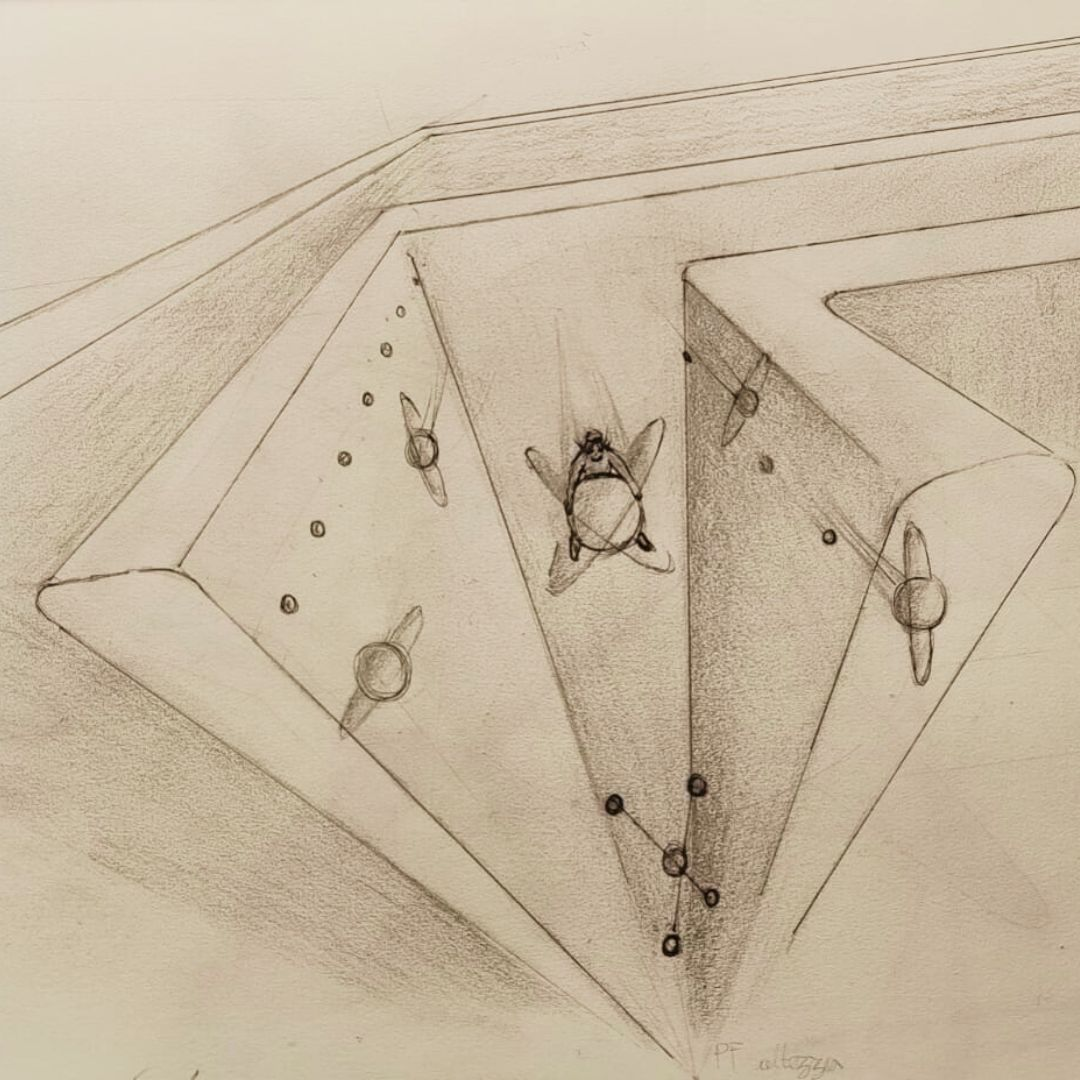
\includegraphics[width=\textwidth]{immagini/cnot_59.jpeg}} % Sostituisci con il nome del file immagine
\end{minipage}
\end{center}

Dietro di loro, l'agente in inseguimento rileva la posizione di Laura e Marley. In un ultimo tentativo di catturarle, modifica la configurazione del suo drone \textit{CH4}. I quattro rotori, precedentemente disposti in formazione tetraedrica, iniziano a ruotare, allineandosi su un unico piano.

\textbf{Allerta:} la nuova configurazione aumenta significativamente la manovrabilità e la stabilità del drone, migliorando la capacità di inseguimento dell'agente. La formazione tetraedrica, che offriva potenza e controllo verticale, è ora sostituita da una disposizione che consente maggiore agilità e velocità orizzontale.

Marley mostra segni di ansia crescente.

\begin{dialogue}
\speak{Marley} \enquote{Laura, sta guadagnando terreno!} esclama.
\end{dialogue}

Laura registra la situazione critica.

\begin{dialogue}
\speak{Laura} \enquote{Credo di avere un asso nella manica,} disse con un sorriso determinato. \enquote{Se riusciamo a imboccare quel diodo nel senso giusto, potremmo passare oltre mentre l'agente resterà bloccato per la polarità inversa. La tecnologia è dalla nostra parte, basta saperla usare.}
\end{dialogue}

Il suo battito cardiaco accelera, ma mantiene la concentrazione. Nonostante la confusione causata dal \textit{gate} di Hadamard, cerca di superare l'instabilità mentale per focalizzarsi sulla fuga e sul salvataggio di Caterina.

La distanza tra i due droni si riduce rapidamente. L'agente ottimizza le traiettorie, anticipando le mosse di Laura.

\textbf{Situazione critica:} se l'agente le raggiunge, la missione di Laura e Marley potrebbe fallire.

Le probabilità di successo diminuiscono. Tuttavia, Laura sfrutta la sua conoscenza dei percorsi interni entrando nel diodo come progettato. L'agente tenta di replicare le sue manovre ma sbaglia polarità e rimane temporanemente bloccato.

\textbf{Tensione massima:} il tempo è essenziale. Laura deve mantenere la lucidità per evitare la cattura. Entrambe le parti spingono al limite le loro capacità, in una corsa contro il tempo.

\begin{dialogue}
\speak{Marley} \enquote{Di la} le dice, indicando l'accesso al Qubit Array, un portale marcato \textbf{Cnot}.
\end{dialogue}
